\section{Metodología}

Para el desarrollo de este proyecto se utilizará la metodología ágil. La ventaja de utilizar esta estrategia de desarrollo sobre otras metodologías lineales (como la metodología de casacada) es que soporta el trabajo simultáneo de varias etapas del desarrollo de software. Esta permite diseñar, desarrollar y probar en pequeños ciclos iterativos hasta que se esté contento con la funcionalidad. Además, el principal objetivo de esta metodología es la entrega de pequeñas partes del proyecto que se complementen entre si \cite{what_is_agile_meth}. Este proyecto se dividirá en los siguientes entregables:

\subsection{Diseño de la red inalámbrica}
La red inalámbrica de sensores tendrá una topología de estrella, donde la computadora central será un \textit{raspberry pi}. Esta será el punto de acceso, servidor DHCP y servidor DNS de los nodos que conformen la red inalámbrica. Se utilizará \textit{Hologram Nova} para acceder a internet a través de una red celular. Esta computadora será la única con acceso a internet.

Los nodos de la red se comunicarán con la computadora central a través de HTTPS. Esto será posible gracias a que esta alojará un API REST que recibirá los datos obtenidos por cada nodo. En la Figura \ref{fig:coms_nodos_raspberry} se puede apreciar un diagrama general de la red inalámbrica de sensores.

\begin{figure}[!ht]
	\centering
	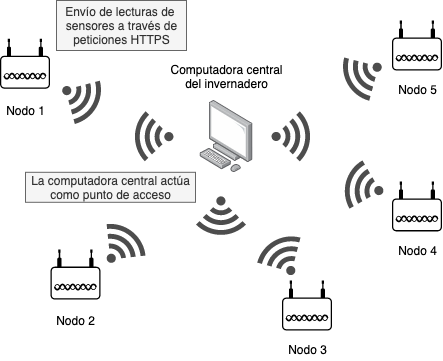
\includegraphics[width=.60\linewidth]{imagenes/diagramas/comunicacion_nodos_raspberry.png}
	\caption{Comunicación entre nodos de la red inalámbrica y la computadora central.}
	\label{fig:coms_nodos_raspberry}
\end{figure}

Se utilizará un microcontrolador Node MCU-ESP826 para sensar los sensores y enviar los datos a la computadora central. Este microcontrolador tiene la ventaja poder utilizarse en una red de malla con hasta 100 metros de distancia entre nodos \cite{nodemcu_mesh}, lo cual es importante considerarlo para determinar la escalabilidad del proyecto. Otra ventaja que ofrece es su modo de ahorro de energía, este permite que el dispositivo entre a un modo de 'sueño profundo' donde su consumo de energía es mínimo \cite{nodemcu_datasheet}. 

Existirán dos variantes de nodos:

\begin{itemize}
    \item Variante 1: Se 
\end{itemize}

\begin{figure}[!ht]
	\centering
	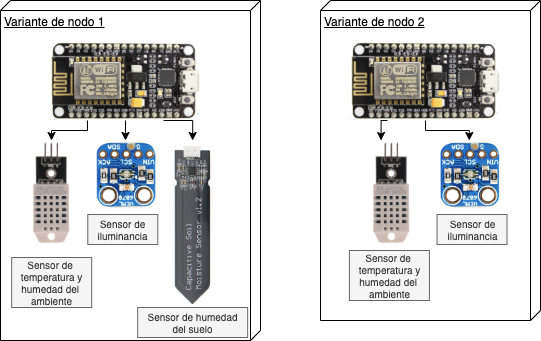
\includegraphics[width=.80\linewidth]{imagenes/diagramas/componentes_nodos_wsn.png}
	\caption{Variantes de nodos con sus componentes.}
	\label{fig:coms_nodos_raspberry}
\end{figure}

\subsection{Desarrollo de la red inalámbrica}


\subsection{Pruebas de la red inalámbrica}
\subsection{Implementación de la red inalámbrica}


\subsection{Desarrollo del API REST de la computadora central del invernadero}
Se desarrollará un API REST para recibir los datos sensados por cada uno de los nodos que conforman la red inalámbrica de sensores y se enviarán al servidor en la nube a través de internet. Los datos recopilados por los nodos serán analizados al momento de ser recibidos para tomar decisiones de control sobre el clima y el riego del invernadero. Este API se estará codificado en Python y se utilizará el \textit{framework} FastAPI. Se probará el API durante el desarollo del mismo.

\subsection{Implementación del API REST de la computadora central del invernadero}
El API REST estará alojado dentro de la computadora central. Se utilizará NGINX como servidor web, este actuará como \textit{proxy} inverso y \textit{buffer} para el servidor de aplicación del API REST. Se utilizará PM2 como manejador del proceso principal del servidor de aplicación. Esto asegurará la disponibilidad de la aplicación. 

\subsection{Desarrollo del API REST del servidor en la nube}
Se desarrollará un API REST para recibir los datos recabados por la computadora central y guardarlos en una instancia de MongoDB. Además, se encargará de la autenticación del cliente web para realizar las consultas de datos históricos y los comandos de control que se tengan que enviar a la computadora central del invernadero. Estará codificada en NodeJS gracias a las bibliotecas disponibles para la integración con la base de datos. Se probará el API durante el desarollo del mismo.

\subsection{Implementación del API REST del servidor en la nube}
El API REST estará alojado en un servidor privado virtual (VPS por sus siglas en inglés) de Digital Ocean. Se utilizará NGINX como servidor web, tanto para el API REST como para la aplicación web. Este actuará como un \textit{proxy} inverso para enviar las peticiones al servidor de la aplicación. Se utilizará el manejador de procesos PM2 para asegurar la disponibilidad del API REST al mantener el servidor de la aplicación siempre disponible. Los componentes que estarán alojados en el servidor en la nube se pueden apreciar en la Figura \ref{fig:componentes_vps}.

\begin{figure}[!ht]
	\centering
	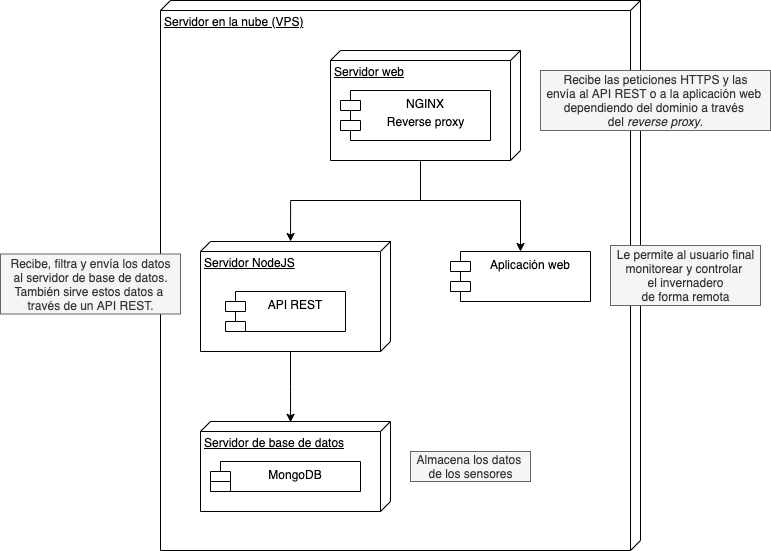
\includegraphics[width=.95\linewidth]{imagenes/diagramas/componentes_vps.png}
	\caption{Diagrama de componentes del servidor en la nube}
	\label{fig:componentes_vps}
\end{figure}



\subsection{Formulación de semántica para razonamiento difuso}
\subsection{Automatización del control mediante técnicas de lógica difusa}



\subsection{Diseño de aplicación web para monitorear y controlar el invernadero de forma remota}
Se harán maquetas de como serán las distintas interfaces del sistema. Se iterará sobre el diseño y la retroalimentación del usuario final. Se contarán con 2 vistas principales, la vista de autenticación y la vista donde se podrá realizar el control y monitoreo. El monitoreo se hará a través de la visualización de la información recabada por los sensores. Una vez que tanto el usuario como el desarrollador estén satisfechos con las interfaces, se procederá a la siguiente etapa.

\subsection{Desarrollo de aplicación web para monitorear y controlar el invernadero de forma remota}
Se utilizará un el \textit{framework} reactivo Vue.js como principal herramienta para el desarrollo de la interfaz. La comunicación con el servidor será a través de Javascript y XML asíncrono (AJAX por sus siglas en inglés) utilizando JSONs como formato para el intercambio de datos. Al consumir el API REST que estará en el servidor en la nube se tendrá acceso a las mediciones históricas de los diferentes sensores y se podrá hacer el control a través del mismo API. Se utilizará un \textit{JSON web token} (JWT) como \textit{token} de acceso al API. Este tendrá que ser enviado en todas las llamadas excepto en la que se utilice para iniciar sesión y obtener el primer JWT. Las pruebas de esta aplicación web se harán durante el desarrollo de la misma.

\subsection{Implementación de aplicación web para monitorear y controlar el invernadero de forma remota}
La aplicación estará alojada en el mismo servidor en la nube que la base de datos y el API REST con el que se recibirán y servirán los datos recopilados por los sensores. Se especifica la interacción con los demás componentes del servidor en la nube en la Figura \ref{fig:componentes_vps}.


% Modelo en cascada

% Análisis 
%     - Los parámetros que les importan a los agricultores los puedo sacar de unas encuestas
% Diseño
%     - Agregar imágenes de los sensores y agregar diagramas de la arquitectura que tendrá el sistema
% Implementación
%     - El microcontrolador se programará en Arduino, los datos se enviarán a través de HTTP
%     - En el rapberry puedo usar python (dependerá de las librerías de lógica difusa)
%     - En el servidor en la nube se utilizará un api en nodejs y se guardarán los datos en Mongo
%     - Para el front se va a utilizar Vuejs, el cual consultará los datos al API en la nube (se va a usar NGINX como servidor web)

%     - 


